\section{eo\-Sorted\-Stat$<$ EOT, Param\-Type $>$ Class Template Reference}
\label{classeo_sorted_stat}\index{eoSortedStat@{eoSortedStat}}
The actual class that will be used as base for all statistics that need to be calculated over the sorted population It's an {\bf eo\-Sorted\-Stat\-Base}{\rm (p.\,\pageref{classeo_sorted_stat_base})} AND an {\bf eo\-Value\-Param}{\rm (p.\,\pageref{classeo_value_param})} so it can be used in Monitors.  


{\tt \#include $<$eo\-Stat.h$>$}

Inheritance diagram for eo\-Sorted\-Stat$<$ EOT, Param\-Type $>$::\begin{figure}[H]
\begin{center}
\leavevmode
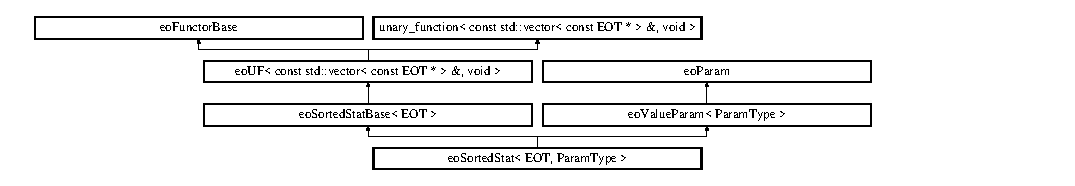
\includegraphics[height=2.04566cm]{classeo_sorted_stat}
\end{center}
\end{figure}
\subsection*{Public Member Functions}
\begin{CompactItemize}
\item 
{\bf eo\-Sorted\-Stat} (Param\-Type \_\-value, std::string \_\-desc)\label{classeo_sorted_stat_a0}

\item 
virtual std::string {\bf class\-Name} (void) const \label{classeo_sorted_stat_a1}

\end{CompactItemize}


\subsection{Detailed Description}
\subsubsection*{template$<$class EOT, class Param\-Type$>$ class eo\-Sorted\-Stat$<$ EOT, Param\-Type $>$}

The actual class that will be used as base for all statistics that need to be calculated over the sorted population It's an {\bf eo\-Sorted\-Stat\-Base}{\rm (p.\,\pageref{classeo_sorted_stat_base})} AND an {\bf eo\-Value\-Param}{\rm (p.\,\pageref{classeo_value_param})} so it can be used in Monitors. 



Definition at line 89 of file eo\-Stat.h.

The documentation for this class was generated from the following file:\begin{CompactItemize}
\item 
eo\-Stat.h\end{CompactItemize}
